

\section{Implementation}
\label{sec:implementation}


The implementation..

\begin{enumerate}
	\item The extra things we did to make the thing actually run
	\item Code architecture
	\item Optimizations
\end{enumerate}



\subsection{Code Architecture}

\label{subsec:codeArchitecture}

The \texttt{ser} crate implements a complete workflow for Petri-net reachability analysis using Presburger arithmetic. From user input to final report, the components collaborate as follows:

\begin{enumerate}
	\item \textbf{Input \& Parsing.} A textual description of a Petri net (places, transitions, initial marking) and optional logical constraints is fed into the parser. The grammar module lexes and parses both net definitions and SMT-style constraint expressions, producing an abstract syntax tree (AST) for each.
	
	\item \textbf{AST to Symbolic Model.} The ASTs are translated into two parallel internal representations:
	\begin{itemize}
		\item A concrete \texttt{Petri<P>} model capturing the graph structure and initial marking.
		\item A symbolic \texttt{PresburgerSet<P>} or \texttt{QuantifiedSet} encapsulating constraints over token counts.
	\end{itemize}
	
	\item \textbf{Semilinear Conversion.} Symbolic sets are normalized into semilinear form (finite union of linear sets). This step tightly couples the Presburger module with the semilinear abstraction, enabling efficient union, projection, and intersection operations.
	
	\item \textbf{Reachability Engine.} The core algorithm invokes a “complement-and-reach” strategy:
	\begin{itemize}
		\item For each semilinear constraint, compute its complement and intersect it with the reachable markings.
		\item Use DNF-style iteration (via \texttt{can\_reach\_presburger}) and recursive pruning to check emptiness.
		\item Optionally delegate heavy Presburger queries to an external SMT/SMPT backend.
	\end{itemize}
	
	\item \textbf{Proof \& Certificate Handling.} If a reachability query succeeds or fails, a proof certificate is generated or consumed. The proof parser reconstructs high-level formulas and associates each algorithmic step with symbolic witnesses.
	
	\item \textbf{Instrumentation \& Logging.} Throughout the pipeline, size and performance metrics (number of places, transitions, constraint complexity, timings) are recorded. The logger outputs structured CSV/JSON logs for later analysis.
	
	\item \textbf{Debug Report Generation.} Finally, a human-readable HTML report is assembled: it embeds the original net, symbolic constraints, reachability results, proof outlines, and profiling graphs. This interactive report allows users to drill down into each transition firing, constraint check, and proof obligation.
	
	\item \textbf{Output Delivery.} The crate exposes a simple CLI and library API. Users obtain either a Boolean reachability verdict (with optional certificate), raw log files, or a full HTML debug report, depending on invocation flags.
\end{enumerate}

%\noindent
%This linear pipeline - \emph{parse} -> \emph{model} -> \emph{normalize} -> \emph{analyze} -> \emph{prove} -> \emph{report} --- ensures a clear separation of concerns, easy extensibility (e.g., swapping backends), and comprehensive traceability from input to certified result.```


\begin{figure}[htbp]
	\centering
	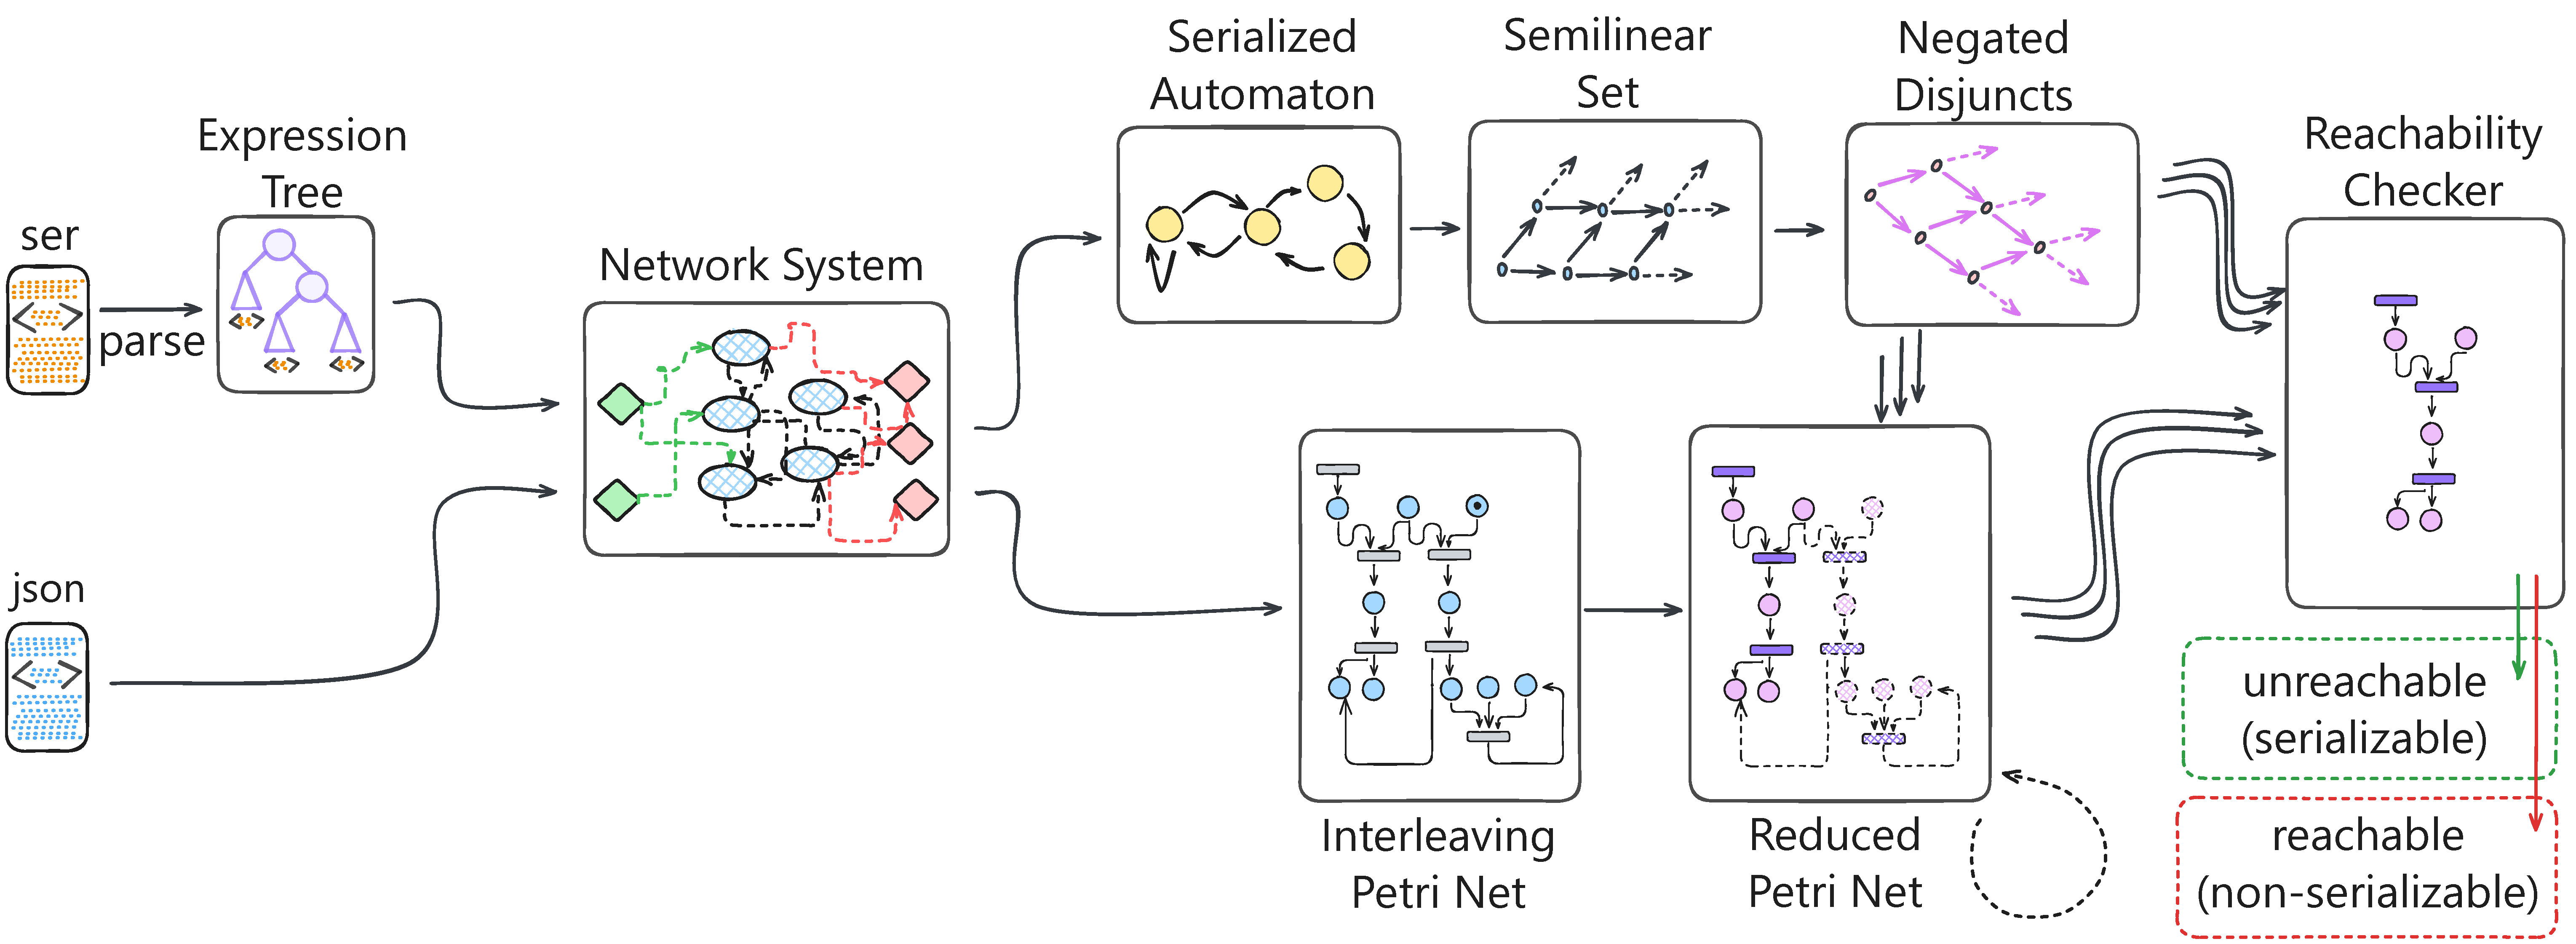
\includegraphics[width=1.0\textwidth]{plots/full_program_flow.pdf}
	\caption{Full program flow. If the program is unreachable --- a serializability proof is produced; otherwise, if it is reachable --- a counterexample trace is generated.}
	\label{fig:full_program_flow}
\end{figure}


\subsection{Optimizations}

\paragraph{Bidirectional Pruning of the Petri Net}
Before any heavy symbolic reasoning takes place, we apply a bidirectional reachability filter to the underlying Petri net.  In the forward pass, we traverse from the initial marking to identify all places and transitions that could ever fire; in the backward pass, we traverse backward from any place that can influence a target constraint, and identify transitions and places that cannot contribute to reaching it.  By iteratively repeating forward passes and backward passes until convergence, we remove every component of the net that cannot both originate and contribute to the reachable target set.  This dramatically shrinks the net in practice, often converting an intractably large model into one small enough for exhaustive analysis.

\paragraph{Redundant‐Constraint Elimination}
When manipulating Presburger sets or their semilinear representations, it is common for some inequalities or disjuncts to add no new coverage beyond what other constraints already guarantee.  The redundant‐constraint elimination pass inspects each linear inequality and each disjunct in a disjunctive normal form, testing whether it is implied by the rest.  Any constraint or disjunct found redundant is dropped, ensuring that subsequent intersection, union, and projection operations work on the smallest necessary formula.  This streamlines the logic formula and prevents exponential blow‐up of case distinctions during solver invocations.
%
%Every time you build or star a semilinear set, you prune out any “period” vectors that are rendered useless by earlier steps:. nce you’ve accumulated a bunch of LinearSet components, you try to merge any that mathematically subsume one another:

\paragraph{Generating Fewer Constraints}
During set‐construction--- especially when introducing new existentially‐quantified variables or combining transition effects, we selectively avoid generating any marking that would strictly dominate an already‐seen solution.  In effect, whenever a candidate disjunct would yield a superset of an existing one, it is skipped entirely.  This ``generate‐less” heuristic stops the proliferation of large, overlapping regions in the semilinear description, trading off completeness of intermediate case‐enumeration for concise final representations.  In benchmarks with large state‐spaces, it can reduce the number of intermediate branches by orders of magnitude.

%in both the Regex and SemilinearSet Kleene-algebra instances. Concretely, instead of always building the full new structure and pruning it later, operations like union (plus) and concatenation (times) do a quick check for trivial cases and drop “zero” or “one” elements on the spo

\paragraph{Doing the Kleene Elimination in a Smart Order:}
When you converting an NFA to a single regex, we pick the next state to eliminate by heuristically choosing the  state with the fewest incoming and outgoing edges.
This optimization allows circumventing 
overblown expressions resulting in naive translations, especially with regard to  Kleene closures (the “\(\mathsf{*}\)” operator).  Instead, we analyze the structure of subexpressions under the various operators --- estimating their branching factor and likely convergence speed, and reorder them so that simpler, low‐branching components are expanded first.  This adaptive ordering often leads to early detection of fixed points or dead‐ends, preventing the combinatorial explosion that arises when complex loops are expanded prematurely.  


\begin{figure}[htbp]
	\centering
	
	% Top row: (a), (b), (f)
	\begin{subfigure}[b]{0.45\textwidth}
		\centering
		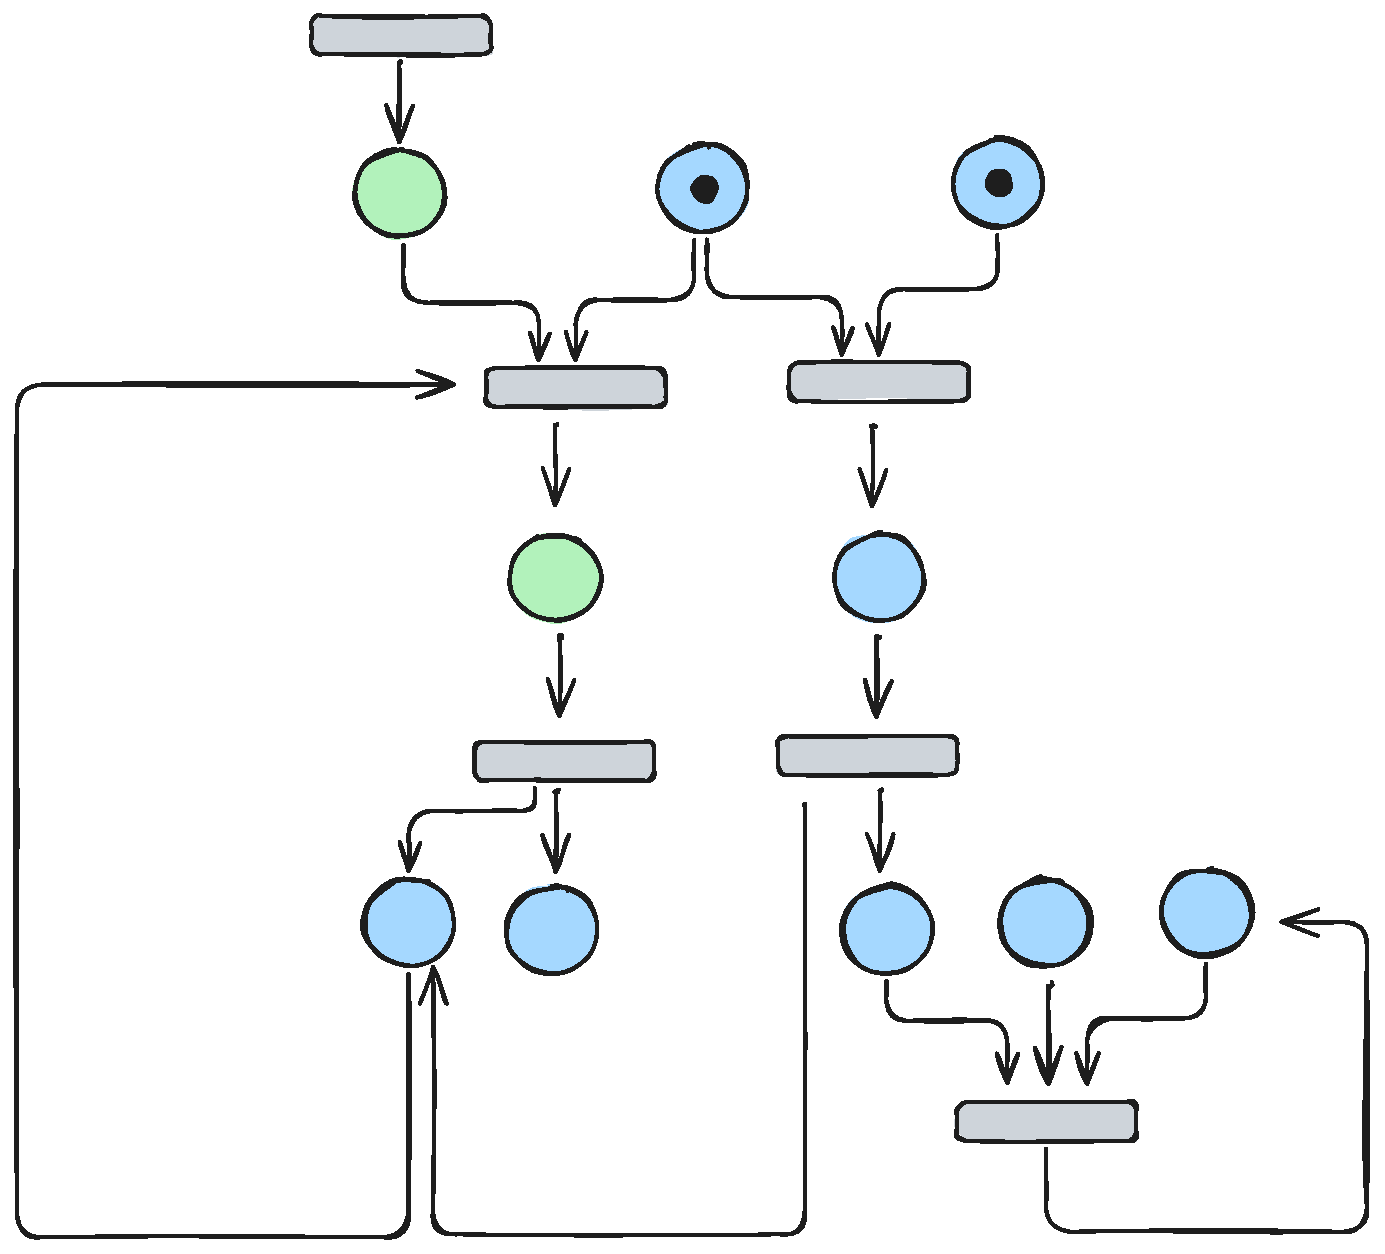
\includegraphics[width=\textwidth]{plots/bidirectional_pruning_step_a_init.pdf}
		\caption{Step 0: initial petri net, before pruning.}\label{fig:step:a}
	\end{subfigure}\hfill
	\begin{subfigure}[b]{0.45\textwidth}
		\centering
		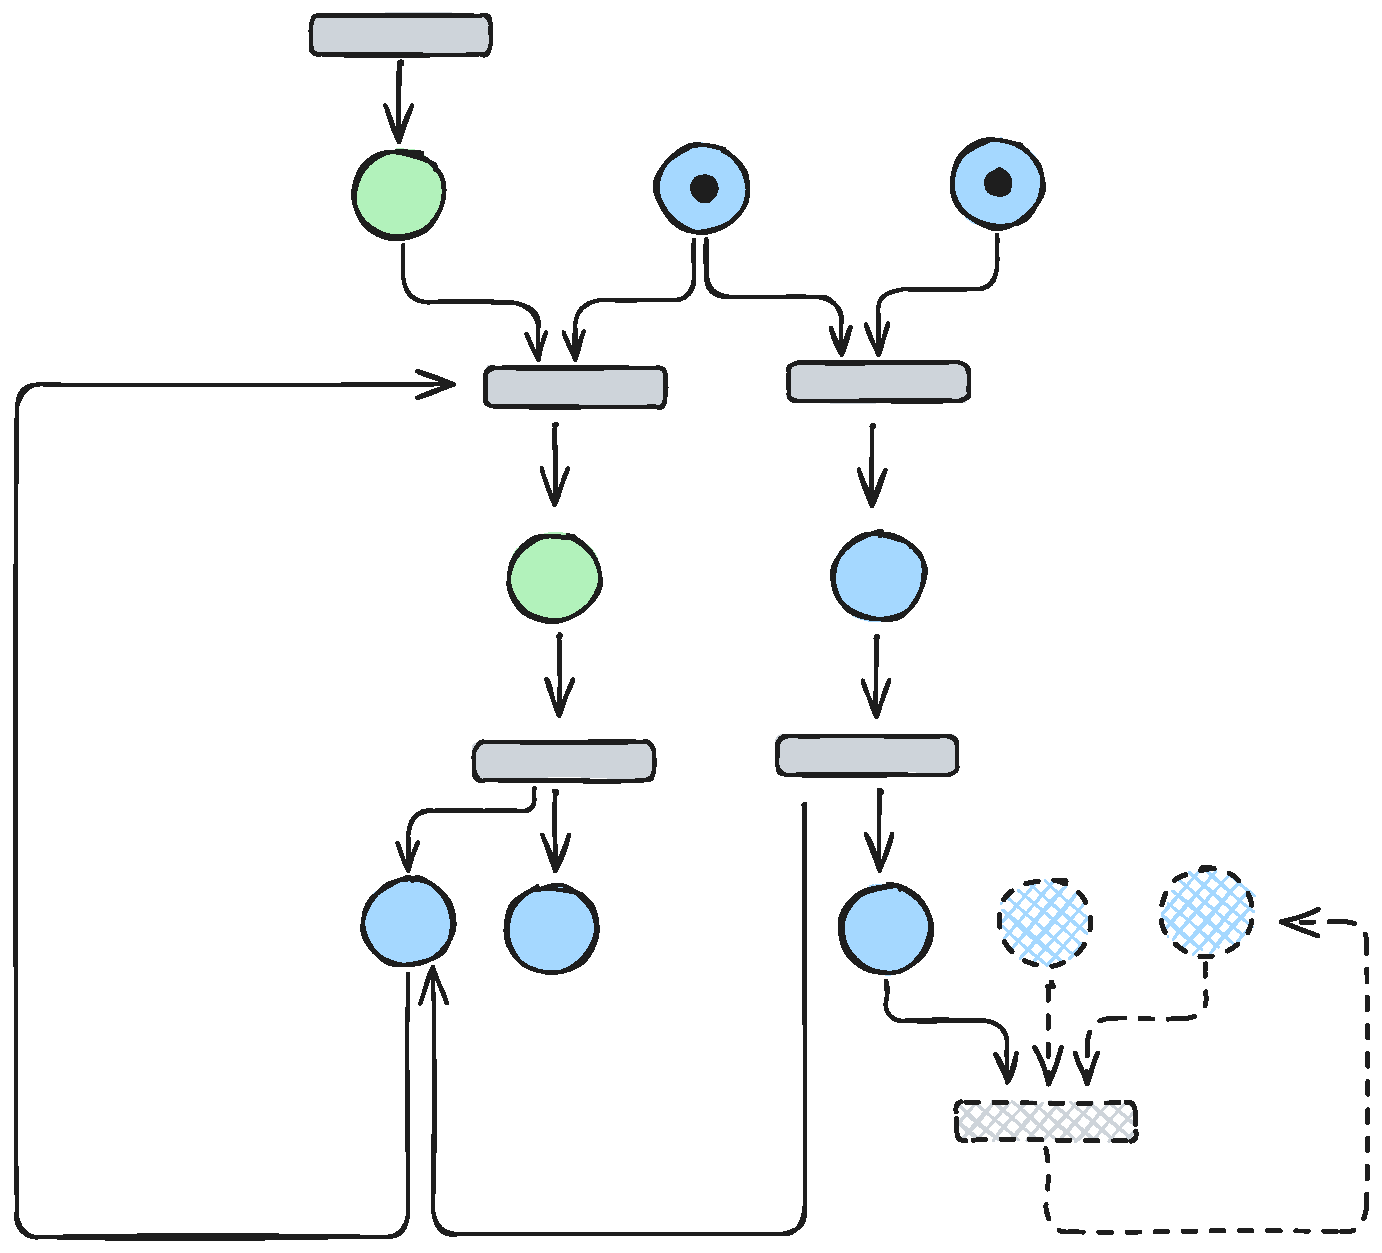
\includegraphics[width=\textwidth]{plots/bidirectional_pruning_step_b_forward.pdf}
		\caption{Step 1: during forward pass.}\label{fig:step:b}
	\end{subfigure}\hfill
	
	
	\vspace{1em}
	
	% Bottom row: (c), (d), then stacked (e)/(f) slot
	\begin{subfigure}[b]{0.30\textwidth}
		\centering
		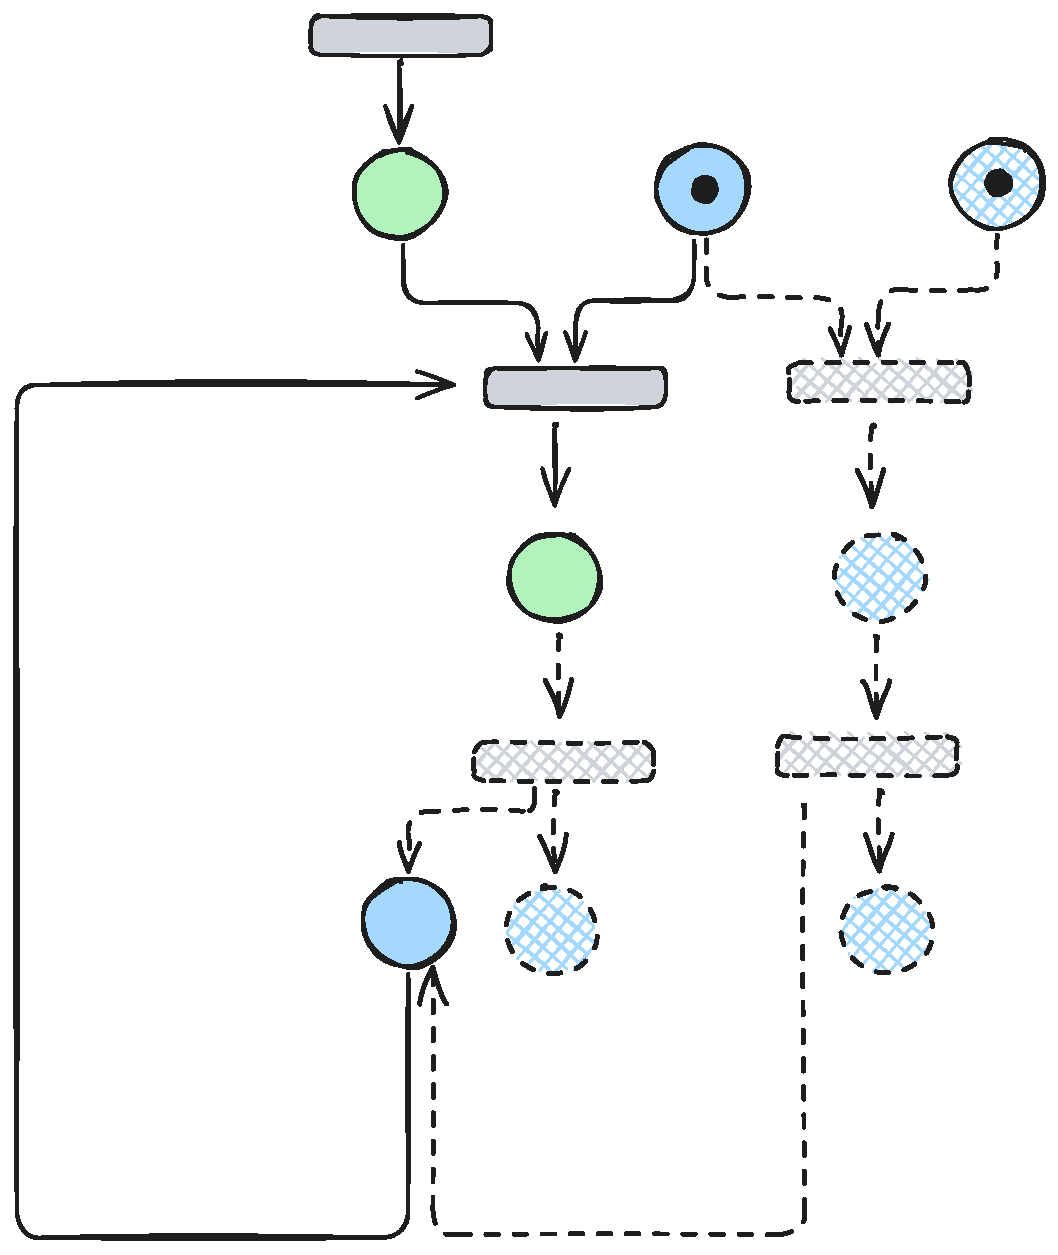
\includegraphics[width=\textwidth]{plots/bidirectional_pruning_step_c_backward.pdf}
		\caption{Step 3: after forward pass, and during backward pass.}\label{fig:step:c}
	\end{subfigure}\hfill
	\begin{subfigure}[b]{0.23\textwidth}
		\centering
		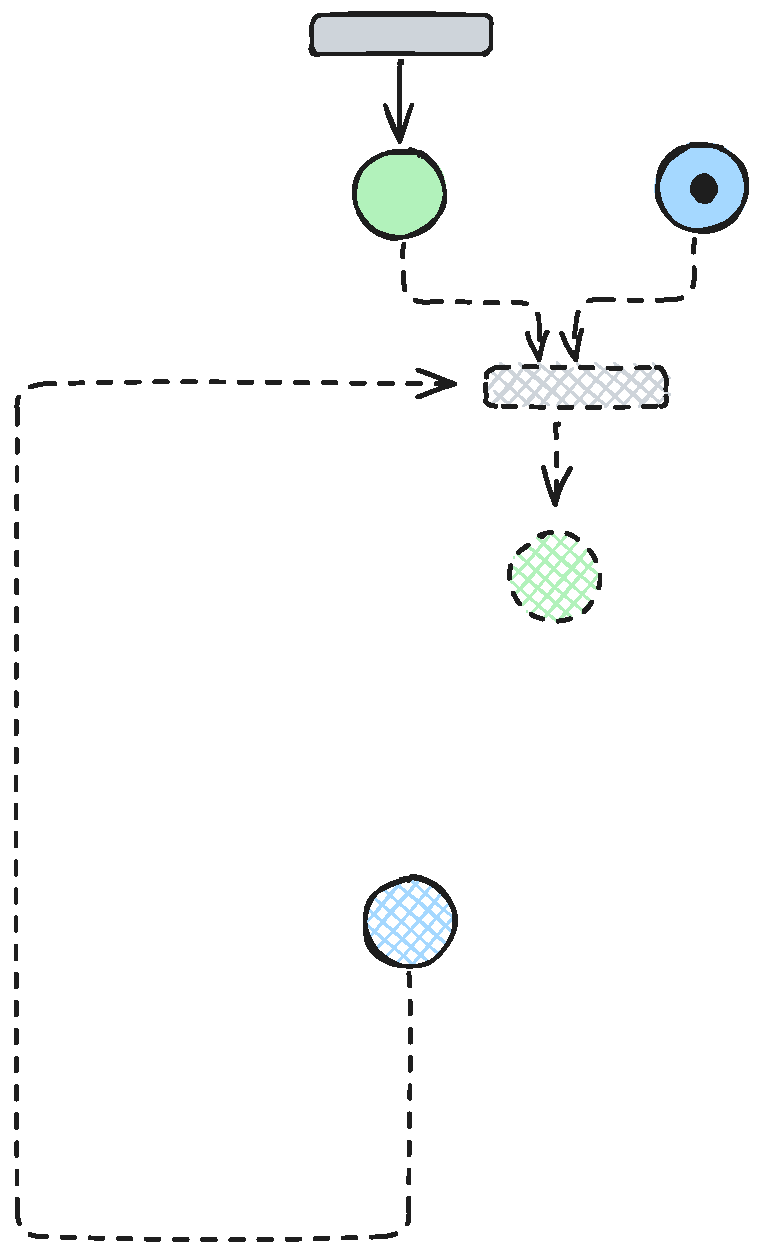
\includegraphics[width=\textwidth]{plots/bidirectional_pruning_step_d_forward.pdf}
		\caption{Step 4: after backward pass, and during forward pass.}\label{fig:step:d}
	\end{subfigure}\hfill
	\begin{subfigure}[b]{0.23\textwidth}
		\centering
		% nested for (e)
		\begin{subfigure}[b]{\textwidth}
		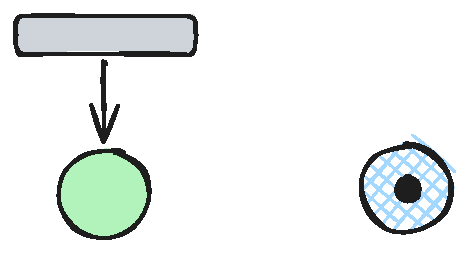
\includegraphics[width=0.5\textwidth]{plots/bidirectional_pruning_step_e_backward.pdf}
			%	       \vspace{-0.5ex}  
%			\raisebox{17ex}{%
%				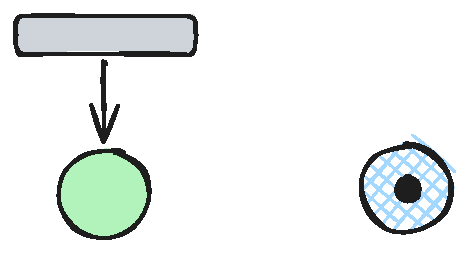
\includegraphics[width=0.65\textwidth]{plots/bidirectional_pruning_step_e_backward.pdf}%
%			}
			%		\captionsetup{skip=-15.5ex}
			\caption{Step 5: after forward pass, and during backward pass.}\label{fig:step:e}
		\end{subfigure}
		
		\vspace{0.5em}
		
		% nested for (f)
		\begin{subfigure}[b]{\textwidth}
			\centering
			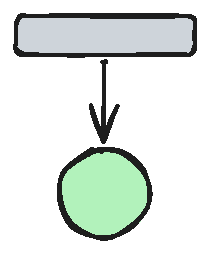
\includegraphics[width=0.23\textwidth]{plots/bidirectional_pruning_step_f_final.pdf}
			\caption{Step 6: final petri net.}\label{fig:step:f:bottom}
		\end{subfigure}
	\end{subfigure}
	
	\caption{A Petri Net after four iterations of bidirectional pruning: two forward passes and two backward passes. Black dots represent initial token markings; green places represent places that are allowed to be reachable in our constraints. Dashed shapes represent places and transitions that are identified as removable in the current iteration, and will be removed after it ends.}
	\label{fig:bidirectional_pruning}
\end{figure}




\newpage